\documentclass[crop,tikz]{standalone}% 'crop' is the default for v1.0, before it was 'preview'
\usepackage{tikz,calc,pgfplots}
\usetikzlibrary{calc}
\begin{document}


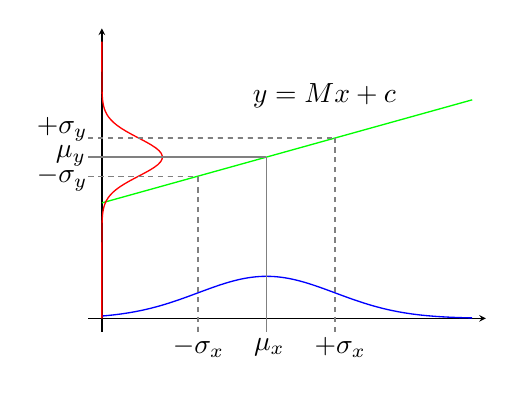
\begin{tikzpicture}[scale=0.6,
declare function={ 
				mu = 6;
				sig = 2.5;
				X(\x) = 1/(sig*sqrt(2*pi))*exp(-((\x-mu)^2)/(2*sig^2)); 				
 				J = 4/(mu*ln(10)); % Jacobian of prop function evaluated at mean value
  				linG(\x) = J*\x+4.38;		
  				sigProp = sig*J; % propagated standard dev
  				muProp = 4*log10(mu)+3; % propagated mean				
  				Yy(\y) = 1/(sigProp*sqrt(2*pi))*exp(-((\y-linG(mu))^2)/(2*sigProp^2));
  			}
]


    \begin{axis}[thick,
		    	 width=10cm,
		    	 height=8cm,
                     samples = 100,
%                     xlabel = $x$,
%                     ylabel = $y$,
                     xmin = -0.5,
                     xmax = 14,
                     ymin = -0.5,
                     ymax = 11,
                     axis x line = middle,
                     axis y line = middle,
%                      axis line style={latex-latex},
                     ticks = none]


                 \addplot[green,domain=-0:13.5] plot (\x, {linG(\x)} );
			  	 \addplot[blue,variable=\x,domain=-0:13.5] plot( {\x} , {10*X(\x)} );            	          
				 \addplot[red,variable=\y,domain=-0:10.5] plot( {4*Yy(\y)} , {\y} );           
           	           	          
				\addplot[gray,dashed,variable=\y,domain=-0.5:{linG(mu+sig)}] plot ({mu+sig}, {\y});
				\addplot[gray,variable=\y,domain=-0.5:{linG(mu)}] plot ({mu}, {\y});
				\addplot[gray,dashed,variable=\y,domain=-0.5:{linG(mu-sig)}] plot ({mu-sig},{\y});  	 

  	          \addplot[gray,dashed,variable=\x,domain=-0.5:{(mu+sig)}] plot ({\x}, {linG(mu+sig)});
   	          \addplot[gray,variable=\x,domain=-0.5:{(mu)}] plot ({\x}, {linG(mu)});
  	          \addplot[gray,dashed,variable=\x,domain=-0.5:{(mu-sig)}] plot ({\x}, {linG(mu-sig)});           	          
            
      \end{axis}

\node at (5.3334,-0.3332) {$+\sigma_x$};
\node at (2.3334,-0.3332) {$-\sigma_x$};
\node at (3.8334,-0.3332) {$\mu_x$};
\node at (5,5) {$y=Mx+c$};
\node at (-0.3666,3.7166) {$\mu_y$};
\node at (-0.5499,4.2834) {$+\sigma_y$};
\node at (-0.5499,3.2331) {$-\sigma_y$};
\end{tikzpicture}

\end{document}